
\subsection{Direction des Études et des Statistiques (DES)}
la Direction des Études et des Statistiques (DES) a pour mission principale de fournir aux autorités de l'Université, aux établissements ainsi qu'aux différentes directions et services, des informations fiables et pertinentes sous forme d'études, d'analyses, de tableaux de bord et d'indicateurs. Ces outils permettent d'éclairer les prises de décisions stratégiques et opérationnelles au sein de l'Université.

La DES est responsable de la collecte, de la centralisation, de la supervision, de l'analyse et de la diffusion des données statistiques de l'UCAD. Elle veille à garantir la qualité, la cohérence et la fiabilité des informations produites, en harmonisant notamment le calcul des indicateurs et en validant, sous l'approbation de la commission de validation, toute production statistique avant communication publique.

En somme la DES facilite la prise de decision au sein de l'Université en fournissant des insights pertinents bases sur une analyse rigoureuse des données. 
\subsection{Mission de la DES} 
Plusieurs divisions existent au sein de la DES, chacune ayant des missions spécifiques :
\begin{itemize}
    \item \textbf{Division planification suivi-Evaluation (DivPSE)} : 
    Leur mission principales sont les suivantes :
    \begin{itemize}
        \item Suivre l'orientation des programmes et projets .
        \item Mettre en oeuvre le suivi de ces programmes et projets.
        \item Produire des rapports de performances des reformes annuelles
    \end{itemize}
    \item \textbf{Division des Études et suivi de la performance } :  
    ils sont chargés de :
    \begin{itemize}
        \item Calculer et mettre a jour les indicateurs de performance
        \item Réaliser des Enquêtes de satisfaction avec la communication .
    \end{itemize}
    \item \textbf{Division des Études Statistiques (DES)} : 
    c'est la division dans laquelle j'ai effectué mon stage. Elle est chargée de :
    \begin{itemize}
        \item Produire la section de l'annuaire statistique de l'UCAD.
        \item Collecter, traiter et analyser les données statistiques 
        \item Soutenir le development des systèmes de collectes de données .
        \end{itemize}
    
\end{itemize}   

voici un organigramme de la DES  et ses divisions :
\begin{figure}
    \centering
    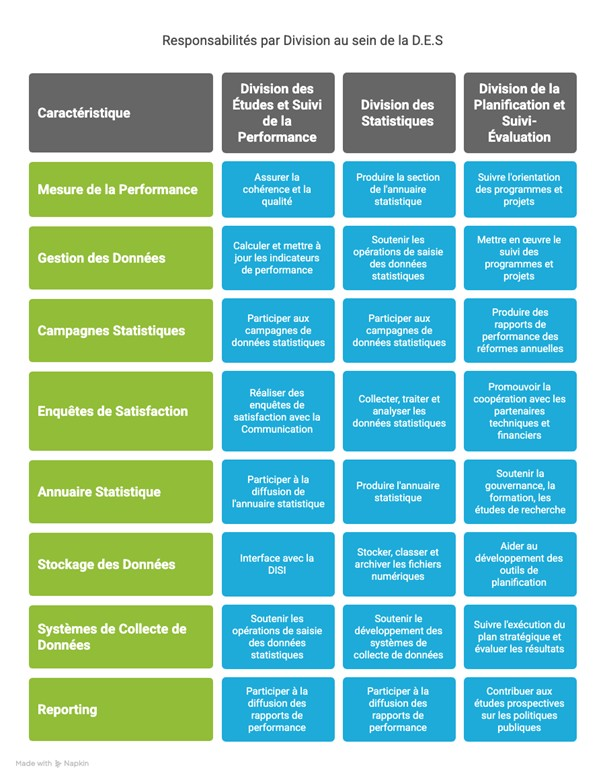
\includegraphics[width=0.8\textwidth]{image/des.jpg}
    \caption{Organigramme de la Division des Études Statistiques (DES)}
    \label{fig:organigramme_DES}
\end{figure} 